\chapter{Introduction}

Els expenedors automàtics de begudes fredes tenen una vida útil bastant llarga però les compres amb efectiu s'estan quedant enrere.

Cada dia el nombre de transaccions amb efectiu es van reduïnt. Els diners en efectiu ocupen espai i, sobretot les monedes, pesen molt. És per això que les transaccions s'encaminen cap al \textit{cashless} (en anglès, sense efectiu).


\begin{figure}
	\centering
	\begin{subfigure}[b]{0.45\textwidth}
		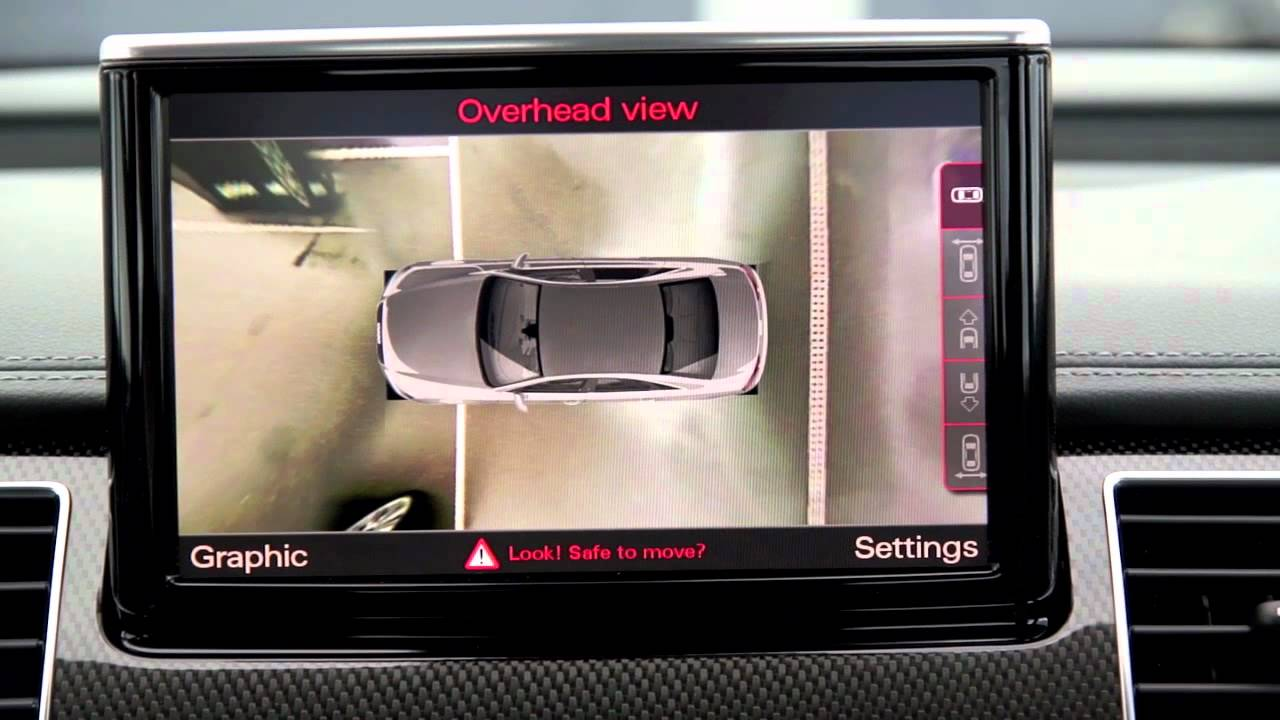
\includegraphics[width=\textwidth]{images/audi-intro}
		\caption{Audi S8 -- 360 View Camera}
		\label{fig:audi-intro-example}
	\end{subfigure}
	\hspace{0.5cm}
	\begin{subfigure}[b]{0.45\textwidth}
		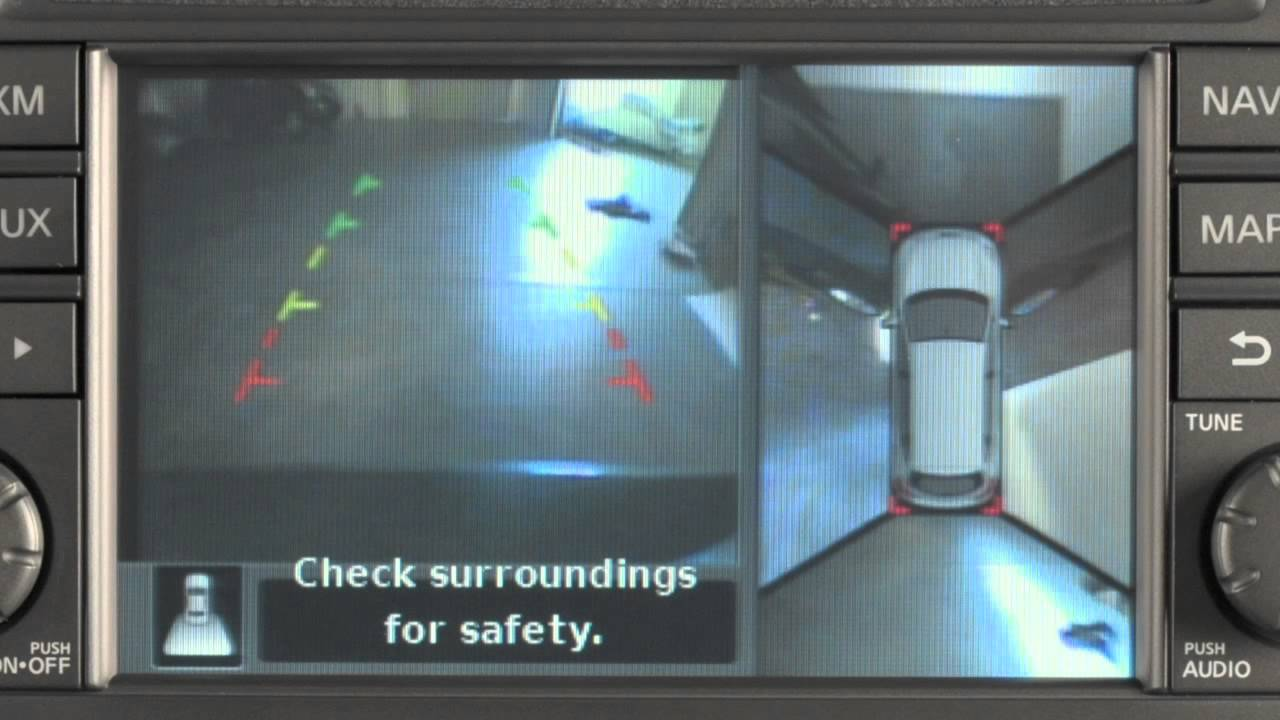
\includegraphics[width=\textwidth]{images/nissan-intro}
		\caption{Nissan Rogue -- Around View Monitor}
		\label{fig:nissan-intro-example}
	\end{subfigure}
	\caption{Two commercial 360\degree~vision systems display view}
	\label{fig:intro-example}
\end{figure}

\section{Objectius del projecte}
The work done in the Image Processing Group started on February 2014. As stated on the Project Proposal and Workplan delivered on February 14th, this TFG work will end at June 30th, although the work in the ARCOL project will be still in development until December 2014.

This project goals had been defined before the development began, and are stated in the Project Proposal and Workplan mentioned above. The goals of this project can be summed up in the following points:
\vspace{-0.5em}
\begin{description}[font=\normalfont\textsl]
\item [Representative points automatic detection.] To perform the stitching a reference points set had to be highlighted on the image. One of this project goals is to define this points and the model shown to each camera on the calibration step.
\item [Estimate the warping parameters. ] Study the most suitable transformation and the parameters needed to deform the input images to obtain the output stitched image.
\item [Blending the results on the final stitching. ] Define an algorithm to merge the warped images on the final composition.
\item [Follow the requirements stated by the Arcol project. ]All the procedures stated before have to be done according with the Arcol UPC project requirements. This requirements and specifications can be found in Chapter~\ref{chapter:requirements}. 
\end{description}

The work done in this five months has been focused on developing a proper warping algorithm for this specific environment, taking into account all the technical an logistic issues. The specific tasks that had been included in  this project scope are explained in Chapter~\ref{chapter:methodology}.

\section{Planificació del temps}

The time plan followed during this project development is shown in Figure~\ref{fig:gantt} Gantt Diagram. The developed work has been split in 8 work packages. A detailed description of each work package and the internal tasks developed can be found on Appendix~\ref{app:gantt}. 

\begin{figure}[ht]
\center
\begin{ganttchart}[
hgrid,
bar/.append style={fill=blue!50},
vgrid={*4{dotted},*1{dashed},*3{dotted},*1{dashed},*3{dotted},*1{dashed},*3{dotted},*1{dashed},*4{dotted},*1{dashed}},
x unit=0.47cm,
title height=1, 
y unit title=0.6cm,
y unit chart=0.8cm]{1}{22}
\gantttitle{Project timeline in months/weeks}{22} \\
\gantttitle{FEBR}{4}
\gantttitle{MARCH}{5}\gantttitle{APRIL}{4}\gantttitle{MAY}{4}\gantttitle{JUNE}{5} \\
\gantttitle[title label node/.append style={below left=-8pt and -7pt}]{\footnotesize\textit{Week}\quad1}{1}
\gantttitlelist
{2,...,22}{1} \\ 
\ganttbar{Training}{1}{6} \\
\ganttbar{System Design}{5}{8}\\
\ganttbar{System Development}{9}{17} \\ 
\ganttbar{Test Unit Design}{18}{18}\\ 
\ganttbar{Test Unit Development}{19}{20}\\
\ganttbar{Writing}{21}{22}
\end{ganttchart}
\caption{Project Gantt Chart}
\label{fig:gantt}
\end{figure}








